\section{File Structure}
\subsection{JSON structure}
The JSON files containing the configurations of the various prediction algoirthms must be structured in the following way

\subsubsection{Support Vector Machine}
\begin{itemize}
	\item \textbf{author}: ;
	\item \textbf{version}: ;
	\item \textbf{algorithm}: ;
	\item \textbf{date}: ;
	\item \textbf{predictors}: ;
	\item \textbf{result}: .
\end{itemize}
\begin{figure}[H]
\centering
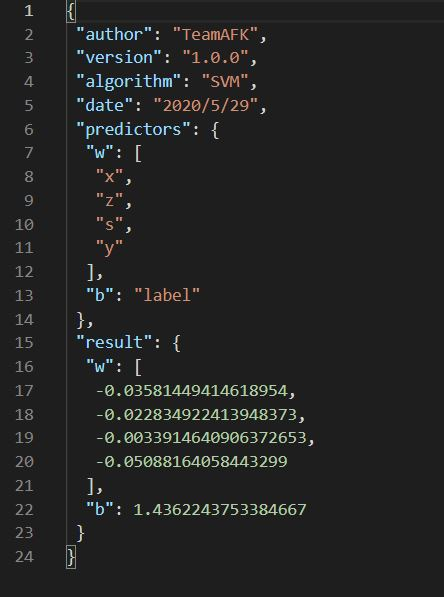
\includegraphics[scale=0.65]{img/json/jsonSVM.jpg}
\caption{Support Vector Machine JSON example}
\end{figure}
\newpage

\subsubsection{Linear Regression}
\begin{itemize}
	\item \textbf{author}: ;
	\item \textbf{version}: ;
	\item \textbf{algorithm}: ;
	\item \textbf{predictors}: ;
	\item \textbf{result}: ;
	\item \textbf{line}: .
\end{itemize}
\hspace{5cm}\\
\begin{figure}[H]
\centering
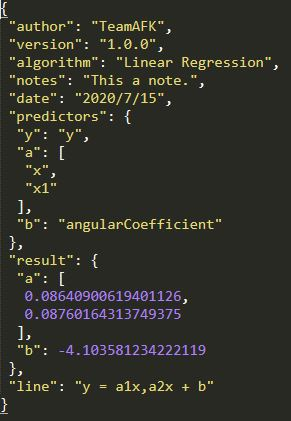
\includegraphics[scale=0.75]{img/json/jsonRL.jpg}
\caption{Linear Regression JSON example}
\end{figure}

\subsection{CSV File structure}
The CSV files are structured based on which algorithm must be trained, RL or SVM.
Each column conains the values of the corresponding predictor\glo.

\begin{figure}[H]
\centering
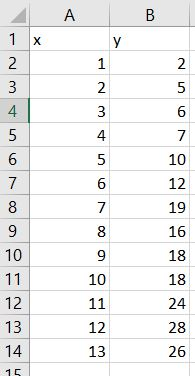
\includegraphics[scale=0.75]{img/json/csvfile.jpg}
\caption{CSV file example}
\end{figure}
